\documentclass[aspectratio=169,11pt]{beamer}

\usepackage[T1]{fontenc}
\usepackage{lmodern}
\usepackage{graphicx}
\usepackage{tikz}
\usetikzlibrary{positioning,arrows.meta}

\definecolor{DeepNavy}{HTML}{13263A}
\definecolor{WarmGold}{HTML}{D9A441}
\definecolor{SoftBlue}{HTML}{EAF1F7}
\definecolor{SoftGold}{HTML}{FFF4D6}
\definecolor{Ink}{HTML}{1E2933}
\definecolor{Muted}{HTML}{5D6B78}
\definecolor{AlertRed}{HTML}{9D2C2C}
\definecolor{Green}{HTML}{2F6F4E}

\setbeamercolor{normal text}{fg=Ink,bg=white}
\setbeamercolor{structure}{fg=DeepNavy}
\setbeamercolor{frametitle}{fg=white,bg=DeepNavy}
\setbeamercolor{title}{fg=white}
\setbeamercolor{subtitle}{fg=SoftBlue}
\setbeamercolor{block title}{fg=white,bg=DeepNavy}
\setbeamercolor{block body}{fg=Ink,bg=SoftBlue}
\setbeamercolor{alertblock title}{fg=white,bg=AlertRed}
\setbeamercolor{alertblock body}{fg=Ink,bg=SoftGold}
\setbeamercolor{exampleblock title}{fg=white,bg=Green}
\setbeamercolor{exampleblock body}{fg=Ink,bg=SoftBlue}
\setbeamercolor{itemize item}{fg=WarmGold}
\setbeamercolor{itemize subitem}{fg=DeepNavy}
\setbeamercolor{enumerate item}{fg=WarmGold}

\setbeamertemplate{navigation symbols}{}
\setbeamertemplate{footline}{%
  \leavevmode%
  \hbox{%
  \begin{beamercolorbox}[wd=.82\paperwidth,ht=2.7ex,dp=1.2ex,leftskip=1em]{author in head/foot}%
    \color{Muted}\small SWOSU Computing Commons \textbullet\ Container Level 0
  \end{beamercolorbox}%
  \begin{beamercolorbox}[wd=.18\paperwidth,ht=2.7ex,dp=1.2ex,rightskip=1em plus1fil]{date in head/foot}%
    \color{Muted}\small \insertframenumber/\inserttotalframenumber
  \end{beamercolorbox}}%
}

\newcommand{\shot}[1]{%
  \begin{center}
  \fbox{\includegraphics[width=0.5\textwidth]{#1}}
  \end{center}
}

\title{Container Level 0}
\subtitle{Build It Here. Run It There.}
\author{SWOSU Computing Commons}
\date{Week 3 \textbullet\ Fall 2026}

\begin{document}

{\setbeamercolor{background canvas}{bg=DeepNavy}
\begin{frame}[plain]
  \vspace{1.0cm}
  {\Huge\bfseries\color{white}Container Level 0\par}
  \vspace{0.35cm}
  {\Large\color{SoftBlue}Build It Here. Run It There.\par}
  \vfill
  {\large\color{WarmGold}The whole idea in one sentence}\par
  \vspace{0.15cm}
  {\Large\color{white}A container is a recipe plus proof that the recipe works
  somewhere else, too.\par}
  \vfill
  {\small\color{SoftBlue}Companion slides for the full recorded walkthrough --
  see the Container Level 0 Canvas page for the video and commands.}
\end{frame}}

\begin{frame}{The five-step workflow}
\begin{enumerate}
  \item Describe an image with a \texttt{Containerfile}.
  \item Build the image with Podman.
  \item Run a container from the image, right here.
  \item Publish the built image to GitHub Container Registry (GHCR).
  \item Pull and run that same image on \emph{another} machine.
\end{enumerate}
\vspace{0.4cm}
\begin{alertblock}{This is Level 0 on purpose}
No web framework, no database, no package manager, no build script --
just enough to see the whole loop once, end to end.
\end{alertblock}
\end{frame}

\begin{frame}{Before you build: check the machine is ready}
\shot{readiness.jpg}
\begin{block}{What to notice}
The recording checks Podman is actually reachable \emph{before} trying to
build anything -- \texttt{podman machine list} / \texttt{podman info}. If
your machine answers with real output instead of a connection error,
you're clear to continue.
\end{block}
\end{frame}

\begin{frame}[fragile]{The whole recipe is two lines}
\shot{containerfile.jpg}
\begin{exampleblock}{The \texttt{Containerfile}}
\begin{verbatim}
FROM docker.io/library/alpine:latest
CMD ["echo", "Hello, world!"]
\end{verbatim}
\end{exampleblock}
\end{frame}

\begin{frame}{Read it one line at a time}
\footnotesize
\begin{center}
\fbox{
\includegraphics[width=0.4\textwidth]{cmd_line.jpg}}
\end{center}
\begin{block}{\texttt{FROM}}
Start from an existing image (\texttt{alpine:latest}) instead of building
an entire filesystem by hand.
\end{block}
\begin{block}{\texttt{CMD}}
The command the container runs the moment it starts: \texttt{echo "Hello,
world!"}.
\end{block}
\end{frame}

\begin{frame}{Build it, then run it}
\footnotesize
\begin{center}
\fbox{
\includegraphics[width=0.4\textwidth]{build.jpg}}
\end{center}
\begin{block}{Build}
\texttt{podman build --tag \$imageName .} turns the Containerfile into an
image and stores it locally.
\end{block}
\begin{block}{Verify first}
The script re-reads the Containerfile and compares it to the expected
recipe \emph{before} building -- catch a typo before it costs you a build.
\end{block}
\end{frame}

\begin{frame}[fragile]{Run it -- proof the image works}
\footnotesize
\begin{center}
\fbox{
\includegraphics[width=0.4\textwidth]{run_pass.jpg}}
\end{center}
\begin{exampleblock}{Success looks like this}
\begin{verbatim}
HELLO_FROM_OUR_OWN_IMAGE
CONTAINER LEVEL 0: PASS
\end{verbatim}
\end{exampleblock}
The container printed the exact text baked into the \texttt{CMD} line.
That's the whole proof at this stage: build here, run here.
\end{frame}

\begin{frame}{Tag it for the registry}
\shot{tag.jpg}
\begin{block}{Tagging does not rebuild the image}
It gives the \emph{same} image a second name -- one your local machine
understands (\texttt{localhost/container-level-0:latest}) and one GHCR
understands (\texttt{ghcr.io/\textless your-username\textgreater/container-level-0:latest}).
\end{block}
\end{frame}

\begin{frame}[fragile]{Login and push -- expect a little friction}
\footnotesize
\begin{center}
\fbox{
\includegraphics[width=0.32\textwidth]{push_friction.jpg}}
\end{center}
\begin{alertblock}{This is normal, not a failure}
A mistyped image path, a scope-limited token, or a first-time
\texttt{podman login} prompt are the most common snags. Catch the exact
error message and fix that one thing -- do not start over from scratch.
\end{alertblock}
\begin{block}{The commands, once the path and token are right}
\begin{verbatim}
gh auth token | podman login ghcr.io -u <user> --password-stdin
podman push ghcr.io/<user>/container-level-0:latest
\end{verbatim}
\end{block}
\end{frame}

\begin{frame}{Run it there -- the payoff}
\begin{center}
\resizebox{\textwidth}{!}{%
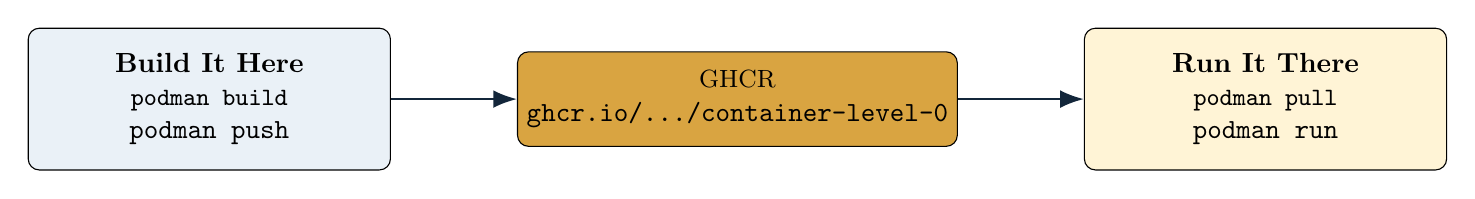
\begin{tikzpicture}[node distance=1.6cm]
  \node[draw,rounded corners,fill=SoftBlue,minimum width=4.6cm,minimum height=1.8cm,align=center] (a)
    {\textbf{Build It Here}\\\small \texttt{podman build}\\ \texttt{podman push}};
  \node[draw,rounded corners,fill=WarmGold,right=1.6cm of a,minimum width=3.0cm,minimum height=1.2cm,align=center] (mid)
    {\small GHCR\\\texttt{ghcr.io/.../container-level-0}};
  \node[draw,rounded corners,fill=SoftGold,right=1.6cm of mid,minimum width=4.6cm,minimum height=1.8cm,align=center] (b)
    {\textbf{Run It There}\\\small \texttt{podman pull}\\ \texttt{podman run}};
  \draw[-{Latex[length=3mm]},thick,DeepNavy] (a) -- (mid);
  \draw[-{Latex[length=3mm]},thick,DeepNavy] (mid) -- (b);
\end{tikzpicture}%
}
\end{center}
\vspace{0.3cm}
\begin{block}{The claim this proves}
The image, not the machine, is the unit of truth. A second computer with
no copy of your source code can still reproduce the exact same output.
\end{block}
\end{frame}

\begin{frame}{Where to go from here}
\begin{itemize}
  \item Full recorded walkthrough and exact commands: Container Level 0
    page, Computing Commons Canvas.
  \item If something goes wrong: see the "If something goes wrong" section
    on that same page -- it lists the real snags from this recording
    (pasted-content parser errors, a stale image after an edit, a
    403 on push, private-by-default visibility).
  \item Using Docker instead of Podman? Same commands, \texttt{docker}
    instead of \texttt{podman} -- see the page for the exact pull command.
\end{itemize}
\vspace{0.4cm}
\begin{exampleblock}{Next step}
Try it yourself: change the \texttt{CMD} line, rebuild, rerun, and watch
the output change. That's the whole loop, in your own hands.
\end{exampleblock}
\end{frame}

\end{document}
